% !TEX root = ../main.tex
\chapter{Introduction}\label{ch:chapter1} % For referencing the chapter elsewhere, use \ref{Chapter1}

%----------------------------------------------------------------------------------------
Video is the medium to record, copy, playback, broadcast
and display the motion images in an electronic style~\parencite{RN190}.
Watching videos is becoming an important way for human entertainment as well
as education.
The high definition (HD) and ultra high definition (UHD) videos
are increasingly demanding nowadays.
People prefer videos with higher resolution than those with lower
resolution because HD videos provide better watching experience.
However, challenges emerged for delivering videos with high definition.
HD/UHD videos typically contain much more information in every
picture frame than videos with lower resolution.
More data needs to be squeezed into the same capacity for transmission.
For example, the uncompressed video with the dimension \(720\times480\) at 30 frames
per second requires 0.03 gigabytes per second, while the uncompressed video with
the dimension \(2880\times2048\) at 120 frames per second requires 2.12 gigabytes per
second.
Since bitrate is proportional to system bandwidth for
transmission~\parencite{RN191}, and heavily expanding the
bandwidth is usually expensive, the significantly increased bitrate
for transmitting the video data is becoming one of the
major obstacles for HD video services.

To cope with the growing need for higher compression of moving
pictures~\parencite{RN193}, Joint Collaborative Team on Video
Coding (JCT-VC)~\parencite{RN192} has finalized the High Efficiency Video
Coding which is the newest international video coding standard for
substantially ameliorate the compression performance against the previous
standards.
Comparing with H.264 Advanced Video Compression Standard~\parencite{RN194},
H.265 High Efficiency Video Coding Standard provides a reduction 
of fifty percent in terms of bitrate while maintaining the objective
video quality at the same level.

Three-dimensional (3D) video has been introduced to market via lots of ways,
including Blu-Ray disc, cable and satellite transmission, terrestrial
broadcast, and streaming or downloading from the Internet~\parencite{RN118}.
3D video provides the perception of depth information which augments
the vividness of video contents.
Currently most 3D videos in the market are using stereo display technology.
Two similar views, one for left eye, the other for right eye, are presented
at the same time with the multiplexing techniques enabling the
adjustments of video geometry information~\parencite{RN196} to provide
the 3D effect.
Figure~\ref{fig:stereo-display} illustrates the typical system structure for
transmitting videos targeting stereo display.
\begin{figure}
    \centering
    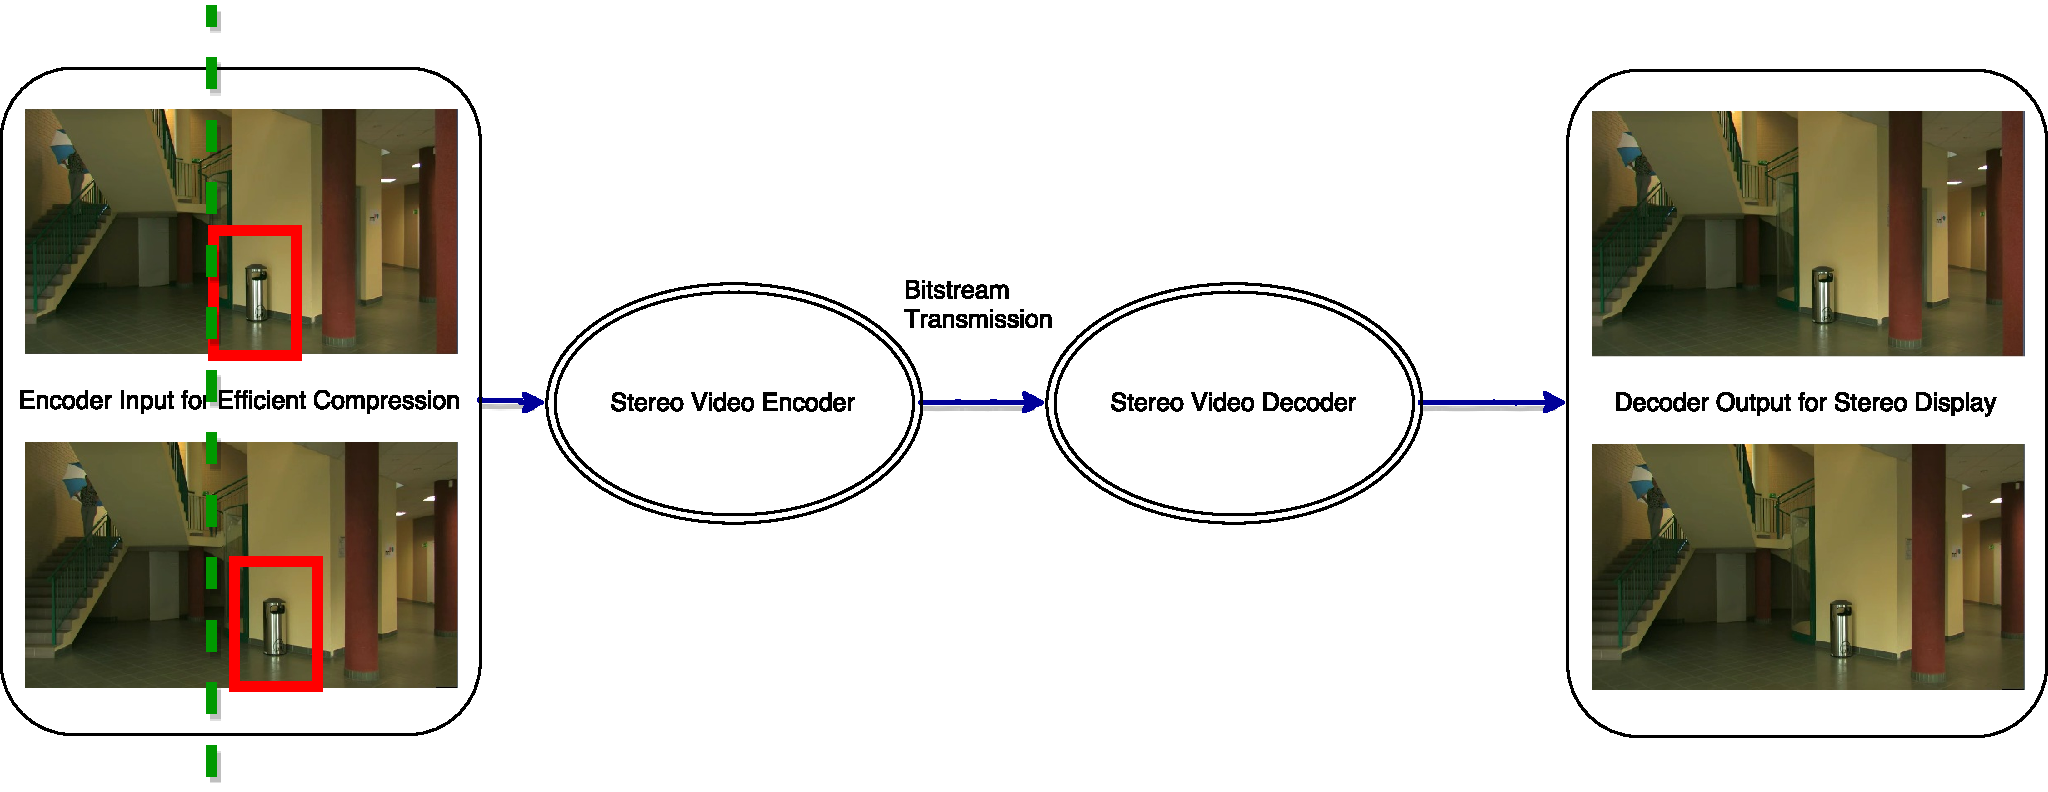
\includegraphics[
        width=\textwidth,
        height=\textheight,
        keepaspectratio
        ]{Figures/StereoDisplay.pdf}
    \caption[System Structure for transmitting videos targeting 
    stereo display]{System Structure for transmitting videos
     targeting stereo display.}\label{fig:stereo-display}
\end{figure}
It can be observed that there exists a displacement between
two views.
The green vertical left margins of the red rectangles in two views
at encoder side are different with each other.
Such a displacement is the visual disparity for 3D perception.
Stereoscopic videos~\parencite{RN153} have
achieved great profitability for movie theatres in recent years.
For example, IMAX 3D has became the most popular one that offering
the immersing multimedia experiences around the world.
Special 3D glasses are needed for watching IMAX 3D movies.
The current 3D film industry is very successful in terms of attracting
customers, however, it is not the end of the story.
Myopic people do not like to wear one more pair of glasses when
watching 3D movies.
Some people will experience discomfort after wearing 3D glasses 
for hours.
To get rid of the undesired 3D glasses,
autostereoscopic multi-view technology~\parencite{RN153} is coming to
the rescue.
The two major different characteristics between stereo display and
autostereoscopic display are
listed in Table~\ref{tab:diff-stereo-autostereo}~\parencite{RN44}.
\begin{table}[b]
    \caption{Comparing characteristics of stereoscopic display and autostereoscopic display}
    \bigskip\label{tab:diff-stereo-autostereo}
    \centering
    \begin{tabular}{c c c}
        \toprule
        Characteristic & Stereo Display & Autostereoscopic Display\\
        \midrule
        Glass-Free & No & Yes \\
        Multiple Stereo Pairs & No & Yes \\
        \bottomrule
    \end{tabular}
\end{table}
The impact of available view amount for autostereoscopic display is shown in
Table~\ref{tab:autostereo-less-views-more-views}~\parencite{RN44}.
\begin{table}
    \caption{The impact of available view amount for autostereoscopic display}
    \bigskip\label{tab:autostereo-less-views-more-views}
    \centering
    \begin{tabular}{c c c}
        \toprule
        Characteristic & Small Number of Views & Large Number of Views \\
        \midrule
        Seamless View Transition  & No & Yes \\
        High Quality of Scene Depth & No & Yes \\
        \bottomrule
    \end{tabular}
\end{table}
Comparative ease can be brought to the 3D video audience
since they do not need to wear 3D glasses for watching autostereoscopic videos.
At each different view position, scenes with minor differences are available
from multiple stereo pairs which are provided by autostereoscopic
display~\parencite{RN44}.
As a result, when audience make moves for various view positions, scenes
not viewable from the previous locations are revealed during the movements.
The autostereoscopic multi-view display demands more than two views.
With a sufficient amount of views present in autostereoscopic display, the
disparities between every two adjacent views can be small enough to offer
seamless transitions from scene to scene, such that when multiple views
meet eyes sequentially, the scenes as a whole can be gorgeous.
The visual quality of the autostereoscopic display is highly proportional to
the number of available views.
Due to limited available bandwidth, transmitting arbitrary number of views
is not practical.
Researchers have proposed a new format which only requires limited number
of views and their associated depth maps for the capability of
generating arbitrary amount of views.
The typical system structure using this new format to compress and supply 3D video
resources is shown in Figure~\ref{fig:SS-MVD}.
An enormous number of views in medium positions which are able to
guarantee the high quality of 3D display can be synthesized from
\begin{figure*}[!b]
    \centering
    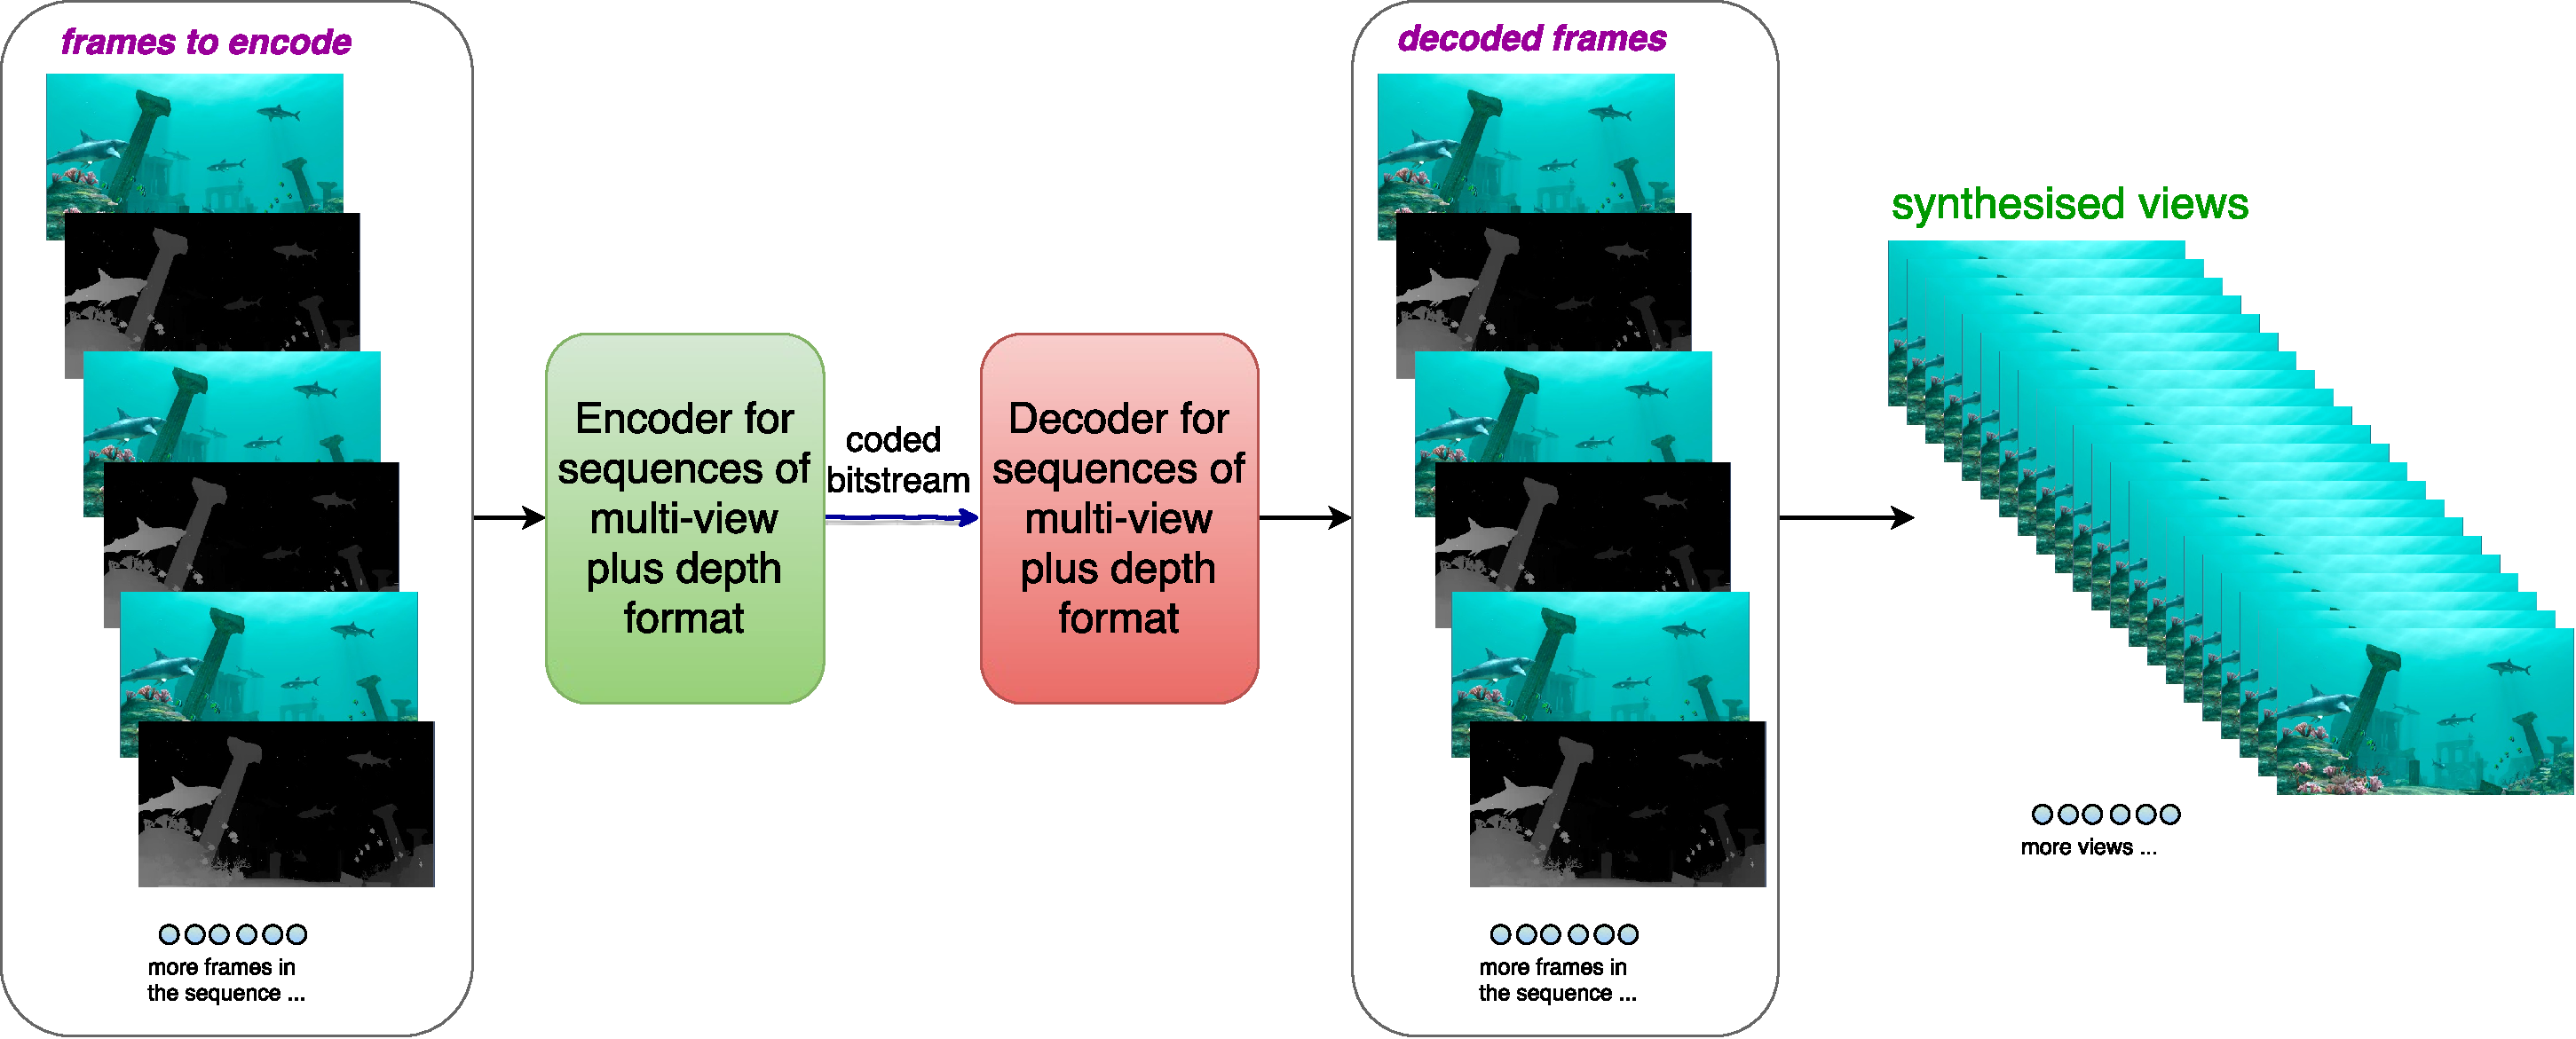
\includegraphics[width=\textwidth,height=\textheight,keepaspectratio]{Figures/SystemStructureOf3DEncoder}
%        \decoRule
    \caption[System Structure for transmitting videos of Multi-view 
    Plus Depth format]{System Structure for transmitting videos of 
    Multi-view Plus Depth format.}\label{fig:SS-MVD}
\end{figure*}
decoded texture frames in combination with decoded depth maps.
%The multi-view plus depth format provides the functionality of synthesizing
%required number of views from texture views and associated depth maps.\\

To employ multi-view plus depth format for 3D video, efficient compressing
methods are needed, which leads to the 3D Extension of
High Efficiency Video Coding Standard (3D-HEVC) by the Joint Collaborative Team
on 3D Video Coding Extension Development (JCT-3V)~\parencite{RN195}.
The 3D Extension of HEVC standard provides extra coding efficiency
for encoding texture views along with the corresponding depth maps by
using new tools. 
Those new tools exploit statistical redundancies between
texture views and depth maps, and pay attention to the unique characteristics of
depth maps, such as large homogeneous
regions separated by sharp boundaries~\parencite{RN47}.

% The distance between distant views
% and nearby views from a static viewpoint,
% can be expressed in the format of depth map.
Depth map vividly conveys the distance between distant views
and nearby views.
\begin{figure*}[!t]
    \centering
    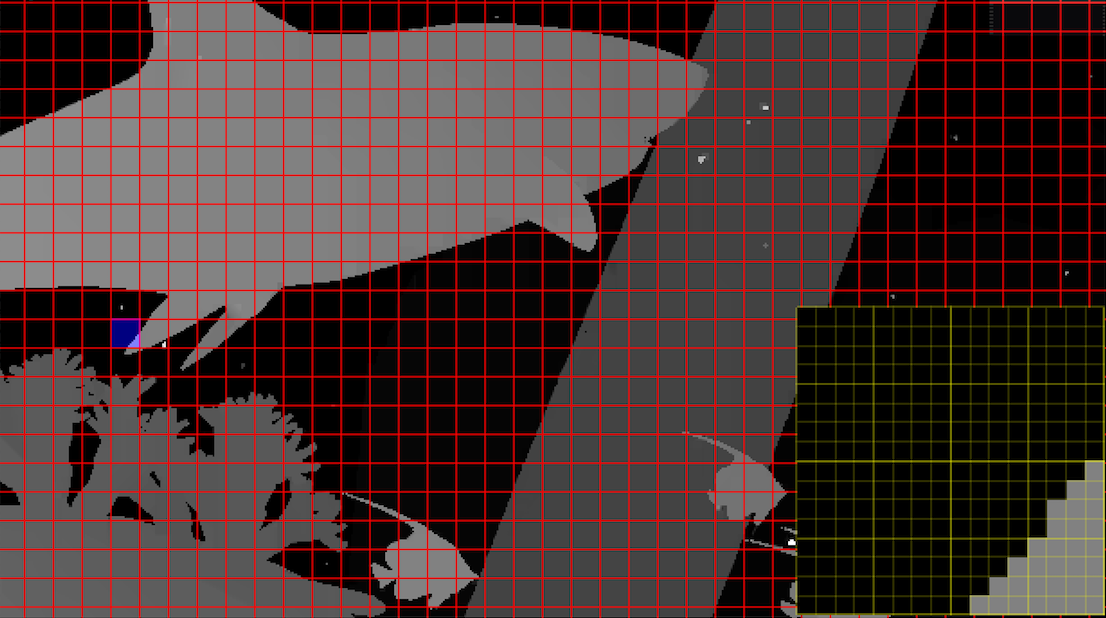
\includegraphics[width=\textwidth,height=\textheight,keepaspectratio]{Figures/wedgelet}
%        \decoRule
    \caption[Wedgelet partition illustration]
    {Example of wedgelet partition in a block of size 
    \(16\times16\) in a depth map
    from Shark video sequence.
    The tiny block highlighted by transparent blue color
    is magnified then shown in the right bottom corner
    of the depth map.
    Wedgelet partitions are straight lines
    that tries their best to fit the sharp edges in CU blocks.
    }\label{fig:wedgelet-partition}
\end{figure*}
Instead of presenting depth maps as 
intermediate views directly to audience, views in the medium
positions are generated by Depth-Image-Based Rendering (DIBR) technique.
The quality of depth maps is vital to the results produced by
DIBR process.
Corona artifacts (a.k.a.\ ringing artifacts)~\parencite{RN44}
can be discovered in synthesized
views if sharpness of edge in depth maps can not be well
preserved.
Therefore, retaining edge sharpness in depth maps is the key to avoid the
artifacts in synthesized views.
There are totally 35 intra-picture prediction modes in HEVC, 
including DC mode, PLANAR mode and 33 Angular modes.
Table~\ref{tab:intra-prediction-tools-in-hevc} 
on page~\pageref{tab:intra-prediction-tools-in-hevc}
specifies 
the indices and names for each of them.
Figure~\ref{fig:intra-angular-modes} 
on page~\pageref{fig:intra-angular-modes} 
illustrates the angle of each 
angular mode.
In 3D-HEVC, all the 35 intra-picture prediction modes
are retained while new intra-picture prediction modes 
and new residual coding methods
have been applied to adapt encoding 
to special properties of depth maps.

\begin{table}[t]
    \caption{Indices and names for each of the intra-picture prediction mode in HEVC}
    \bigskip\label{tab:intra-prediction-tools-in-hevc}
    \centering
    \begin{tabular}{c c}
        \toprule
        Index of mode & Name of mode\\
        \midrule
%        Overall Display Resolution & High & Low \\
        0  & PLANAR \\
        1  & DC \\
        2..34 & Angular (\textbf{X}), \textbf{X} = 2..34  \\
        \bottomrule
    \end{tabular}
\end{table}

\begin{figure}
    \centering
    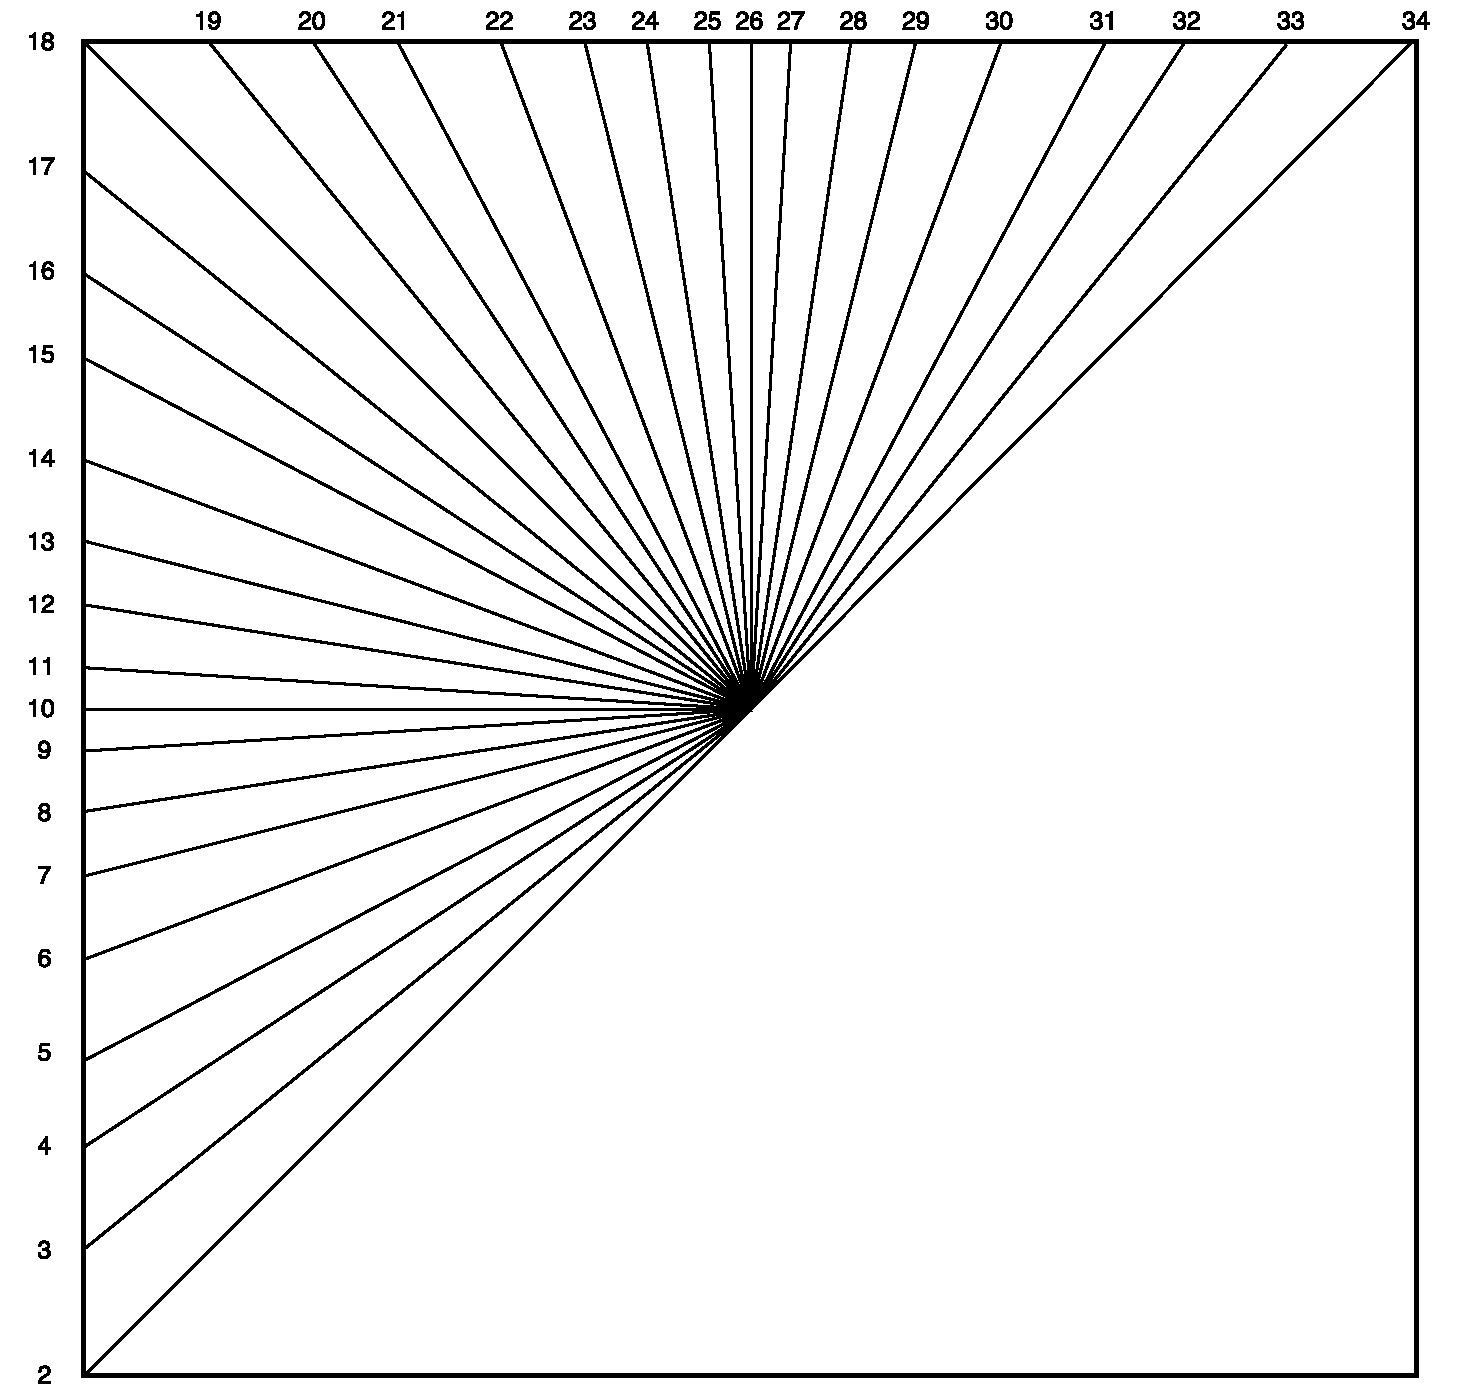
\includegraphics[width=\textwidth,height=\textheight,keepaspectratio]{Figures/intra-angular-modes-in-hevc.pdf}
    \caption[Angular modes in HEVC]
    {Intra angular modes in HEVC\@.
    All the angular modes are pointing to the center of the square.
    The modes adjacent to angular mode 10 and 26 are more dense
    than others to provide more flexibility for encoding vertical
    patterns and horizontal patterns.
    }\label{fig:intra-angular-modes}
\end{figure}


Depth Modelling Mode (DMM), which is one of the new intra-picture
prediction tools, is capable of conserving sharp edges in the shape
of straight line.
It provides a very dense set of straight partitions
which will be looped through in order to find the most suitable candidate
for each in the CU blocks in depth maps.
Figure~\ref{fig:wedgelet-partition} presents an example of wedgelet
partition in a depth map from Shark video sequence.
The small block highlighted by blue color amongst the blocks
separated by the red grid is magnified at the right-bottom position.
Straight lines are used for the partitions in wedgelet mode.
Figure~\ref{fig:contour-partition} shows a sample of the contour partition
from the same depth map shown in Figure~\ref{fig:wedgelet-partition}.
The partition pattern comprises contour line instead of
straight line.
Wedgelet partition and contour partition for depth maps
are enabled by DMM1 and DMM4 separately.
%The wedgelet partition is shown in Figure.
%The contour partition is shown in Figure.
%~\parencite{RN197}.
\begin{figure}
    \centering
    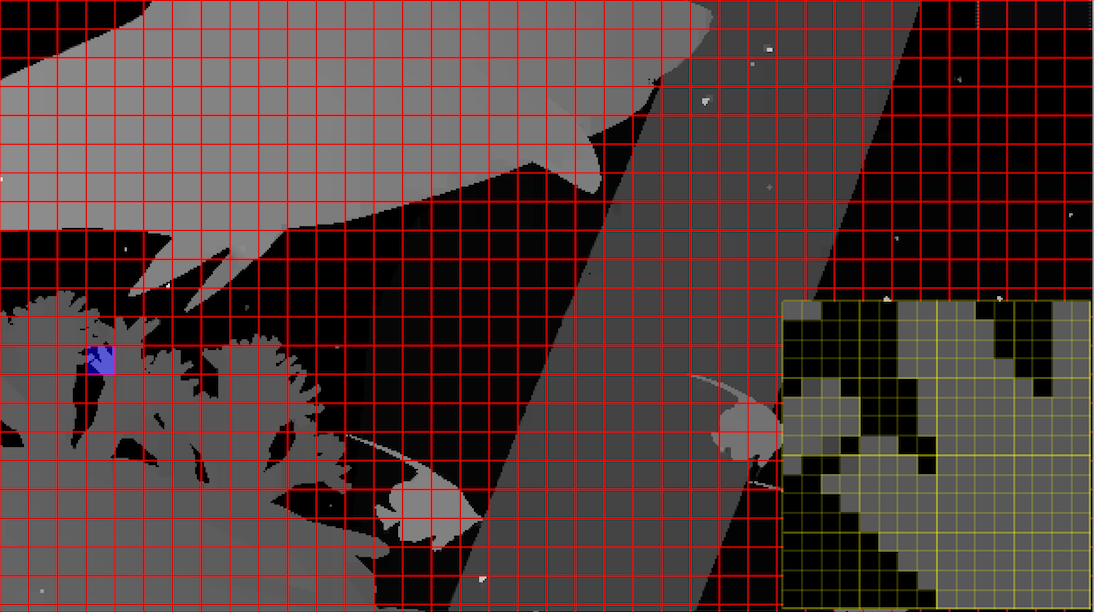
\includegraphics[width=\textwidth,height=\textheight,keepaspectratio]{Figures/contour}
%        \decoRule
    \caption[Contour partition illustration]
    {Example of contour partition in a block of size \(16\times16\) in a depth map
    from Shark video sequence.
    The tiny block highlighted by transparent blue color
    is magnified then shown in the right bottom corner
    of the depth map.
    Contour partitions are irregular lines
    that tries their best to fit the sharp edges in CU blocks.
    }\label{fig:contour-partition}
\end{figure}
%introduce a little about depth map and their usage.
%mentioning iphonex true depth camera.
%draw the picture

%----------------------------------------------------------------------------------------

\section{Motivation}\label{sec:motivation_and_contribution}
The idea of this work originates from the discovery of computational
complexity inside the process for finding the best wedgelet in DMM1.
The immense intricacy for searching the best wedgelet candidate results in
a massive increase of encoding time.
The time consumed for compressing a single depth map in 3D-HEVC encoder is
roughly a sixfold increase relevant to the encoding time of a single texture
frame wherein All-Intra configuration in \(HTM16.2\) is used.
To reduce the heavy time required in depth map coding, 
a computational model, which is a deep convolutional neural network,
has been designed and trained to predict the most probable angular mode
for each CU block.
The predicted angular mode is utilized to further predict the 
most probable wedgelet candidates.
% Thus a computational model has which has been trained
% for predicting the most probable angular mode, which in turn 
% can help with reducing the complexity in DMM1.
The learned models exhibit 91.9\% to 97.0\% top-15 precision for various
block sizes.
It has been integrated into the reference software
\(HTM16.2\) of 3D-HEVC\@.
The learned models can reduce roughly half of the wedgelet candidates.
It provides 64.6\% time reduction in average while the BD performance
has a negligible decrease comparing with the original
implementation of 3D-HEVC encoder.

\textbf{Motivation for Wedgelet Candidates Reduction:} The time
consumed by the encoder from \(HTM16.2\) for
each view can be observed from command line outputs.

Figure~\ref{fig:encoding-time-example} shows a piece of command line outputs
from the encoding process of Shark sequence.
\begin{figure}
    \centering
    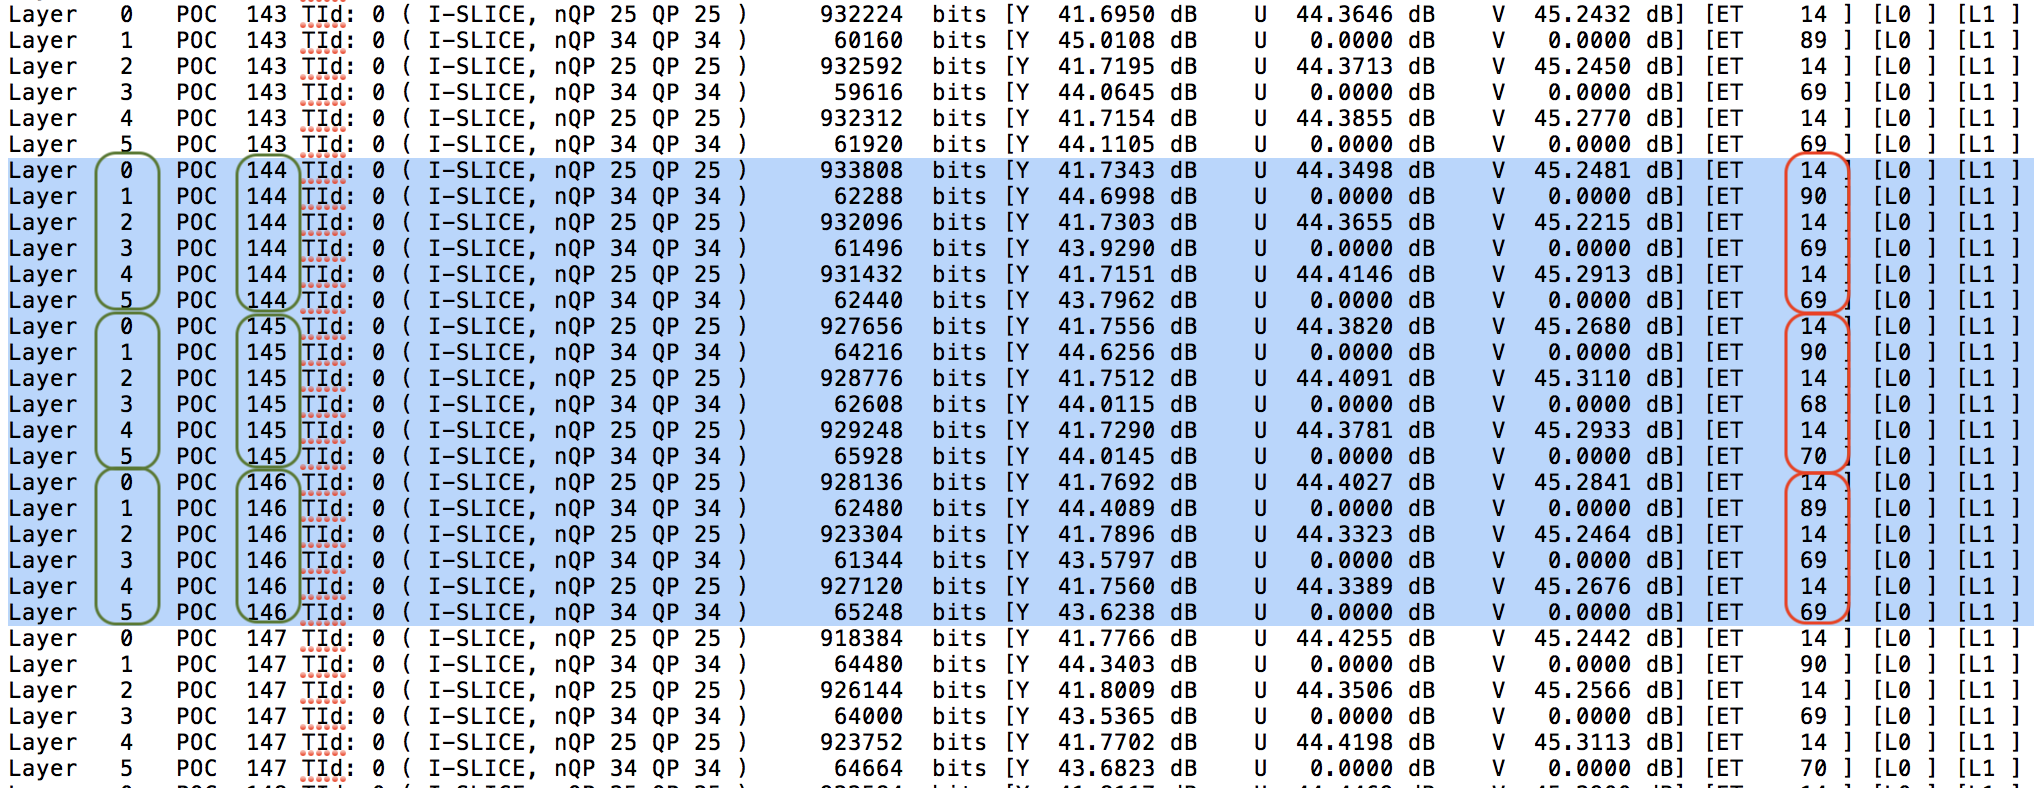
\includegraphics[width=\textwidth,height=\textheight,keepaspectratio]{Figures/EncodingTimeEg}
%        \decoRule
    \caption[An example showing a piece of the command line outputs during
    the encoding process for Shark sequence]
    {An example showing a piece of the command line outputs during the
    encoding process for Shark sequence.
    }\label{fig:encoding-time-example}
\end{figure}
\begin{figure*}[!b]
    \centering
    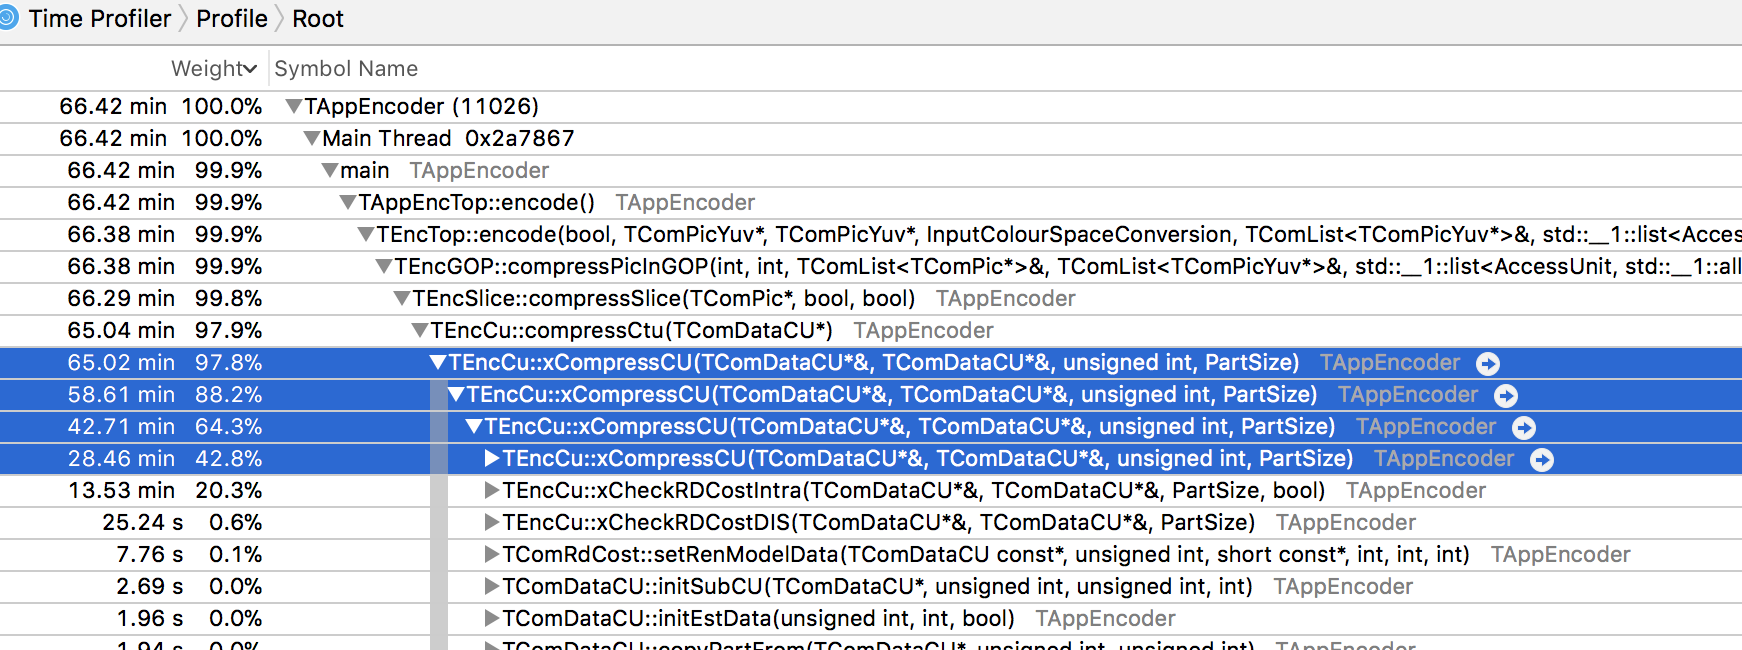
\includegraphics[width=\textwidth,height=\textheight,keepaspectratio]{Figures/major-time-spent-in-recursive-xcompresscu}
%        \decoRule
    \caption[A screen capture of the time profiling information for Newspaper sequence]
    {A screen capture of the time profiling information for Newspaper sequence.
    }\label{fig:major-time-spent-in-recursive-comresscu}
\end{figure*}
The numbers in red blocks stands for the encoding time of certain views, while
the corresponding layer Id and Picture Order Count (POD) are in the green
blocks.
A repetitive pattern of the encoding time for each view can be observed
every six numbers vertically.
A simple calculation using six numbers within the top-most
red block, \((90+69+69)/(90+69+69+14*3) \approx 0.84\), shows that
approximately 84\% total encoding time is busy with encoding
depth maps.
Similarly, it is reported in~\parencite{RN111} that the 
encoding for depth maps
consumes nearly 86\% total 3D-HEVC encoding time.
A trial of time profiling for 3D-HEVC encoder is performed using Instruments
which is an application available on macOS\@.
After encoding the Newspaper sequence for more than one hour,
Figure~\ref{fig:major-time-spent-in-recursive-comresscu} clearly shows
97.8\% time is used to compress the CUs recursively.
The first recursive \textbf{xCompressCU} function 
(denoted as \textbf{XC1} thereafter) is
for CUs of size \(64\times64\), 
the second one
(denoted as \textbf{XC2} thereafter) is targeting 
CUs of size \(32\times32\),
the third one (denoted as \textbf{XC3} thereafter) is dedicated
to CUs of size \(16\times16\), 
and the last one 
(denoted as \textbf{XC4} thereafter) is bound
to CUs of size \(8\times8\).
It can observed from 
Figure~\ref{fig:major-time-spent-in-recursive-comresscu} 
that the most time consuming part
during the process of
compressing depth CUs is DMM1 searching.
The time percentage that DMM1 searching time has in total time occupied 
by \textbf{xCompressCU} is summarized in
Table~\ref{tab:dmm1-searching-time-percent-summary} wherein the summary
for \textbf{XC1} is omitted since DMM1 is not 
applicable to CUs of size \(64\times64\) in
\(HTM16.2\).
\begin{table}[t]
    \caption{The percentages that DMM1 searching time has in total time occupied 
    by \textbf{xCompressCU}}
    \bigskip\label{tab:dmm1-searching-time-percent-summary}
    \centering
    \begin{tabular}{c c c}
        \toprule
        size & xCompressCU & Percentage\\
        \midrule
%        Overall Display Resolution & High & Low \\
        \(32\times32\)  & \textbf{XC2} & 30.0\% \\
        \(16\times16\) & \textbf{XC3} & 25.6\% \\
        \(8\times8\) & \textbf{XC4} & 18.8\% \\
        \bottomrule
    \end{tabular}
\end{table}[t]
The major reason leading to the time consuming property of DMM1 searching is the
View Synthesis Optimization (VSO) Method for improving quality of
synthesized views~\parencite{RN124}, in which the Synthesized View Distortion
Change (SVDC) is computed.
The time percentage that VSO has in DMM1 searching are summarized in
Table~\ref{tab:vso-in-dmm1-searching-time-percent-summary}.
\begin{table}[t]
    \caption{The time percentage that VSO has in DMM1 searching}
    \bigskip\label{tab:vso-in-dmm1-searching-time-percent-summary}
    \centering
    \begin{tabular}{c c c}
        \toprule
        size & Process & Percentage\\
        \midrule
%        Overall Display Resolution & High & Low \\
        \(32\times32\)  & VSO in DMM1 searching from \textbf{XC2} & 80.1\% \\
        \(16\times16\) & VSO in DMM1 searching from \textbf{XC3} & 83.7\% \\
        \(8\times8\) & VSO in DMM1 searching from \textbf{XC4} & 78.8\% \\
        \bottomrule
    \end{tabular}
\end{table}
In \(HTM16.2\), a large number of wedgelet candidates are 
evaluated using VSO which
introduces computational complexity.
Intuitively, evaluating less wedgelet candidates can help with relieving
the heavy burden of computation bared by encoder,
thereby time reduction can be achieved.

\textbf{Motivation for Using Deep Learning:} Deep learning 
is a sub field of representation learning, which
is in turn a major subset of machine learning~\parencite{RN158}.
Machine learning~\parencite{RN198}
has been applied to many scenarios in the domain of Artificial Intelligence (AI).
Deep learning was found hard to proceed further
in the late 1980s~\parencite{RN199}.
However, starting from 2012, it kicks off its
glorious comeback.
The deep Convolutional Neural Network (CNN) has won the ImageNet
Large Scale Visual Recognition Challenge (ILSVRC)
from 2012 to 2015, with the CNN architecture going deeper
and deeper.
The great achievements have attracted attentions from 
people all over the world and
have made deep learning the most popular topic in our daily lives.
Inspired by the fact that supervised deep learning can learn multiple layers of
abstract representations in the visual recognition tasks, it should
be applicable to recognize the angular modes of the intra-picture
prediction in 3D-HEVC\@.
The final DMM1 candidates selected in depth map coding
are essentially determined by the angle pattern of depth blocks.
If we can make use of deep learning to predict the most probable angles of the
target pixel block, a large amount of angular modes and DMM1
wedgelet candidates can be naturally skipped by which the time saving can be
achieved without sacrificing much of the coding performance.

Motivated by the discussions above, we adopt deep learning approach with
deep convolutional neural network to accelerate depth map coding in
3D-HEVC\@.

\section{Contribution and Dissertation Outline}\label{sec:outline}
We accelerate depth map coding using deep learning.
The contributions of the dissertation are:
\begin{itemize}
  \item A deep convolutional neural network with 32 layers 
  comprising ResNet units~\parencite{RN67}
  has been designed and trained to recognize the
  most probable angular mode of coding units (CUs) 
  in intra-picture prediction in 3D-HEVC
  encoder.
  Each learned model has high top-15 precision which works 
  well on tasks of recognizing intra angular patterns in 3D-HEVC\@.
  \item A way of integrating the learned model into \(HTM16.2\) encoder has
  been suggested.
  By making use of Bazel~\parencite{RN200} to compile the encoder binary, the
  data level parallelism (instead of concurrency) functionality in CPU
  as well as the parallel architecture in GPU are fully utilized for
  efficient matrix computations.
  \item An algorithm for fast
  depth map coding
  has been proposed and implemented.
  The simulation results show that the proposed algorithm is capable of
  reducing 64.6\% of encoding time in wedgelet searching during 3D-HEVC encoding process
  while the BD performance only has a trivial decrease.
\end{itemize}
The first two contributions lay the foundation for the third one, which is the
main objective of this work: to accelerate the depth map encoding process in
3D-HEVC\@.

\textbf{Chapter~\ref{ch:chapter2}} supplies the background of video
coding history, video coding standards, and deep learning using artificial
neural networks.
Prior arts in video coding are surveyed in this chapter.

\textbf{Chapter~\ref{ch:chapter3}} describes the algorithm which has been
implemented to collect the data to be used in deep learning.
Data pre-processing steps are described in detail along with
the reasons behind the scene. 
A rich set of visualizations are presented to illustrate 
the properties of the collected data.
% Collected data are visualized to
% understand their properties which can further 

\textbf{Chapter~\ref{ch:chapter4}} presents a deep convolutional
neural network which has been applied in our deep learning.
Both architecture and settings
are covered in detail.
The stopping criteria are shown with the training results.
At the end of the chapter, the evaluation results for learned models
are presented.

\textbf{Chapter~\ref{ch:chapter5}} 
shows the methods
used to integrate learned models
into the reference software of 3D-HEVC\@.
The problem encountered during the integration is described,
and the solution for the problem is presented.
Simulation results comparing with the original \(HTM16.2\) are given in this
chapter.

\textbf{Chapter~\ref{ch:chapter6}} concludes the thesis.
